% vim: set tw=78 aw sw=2 sts=2 noet:

\section{Image classification}

\begin{frame}{Supervised learning}
Machine learning paradigm in which an algorithm learns from labeled data to
make predictions
  \begin{figure}
	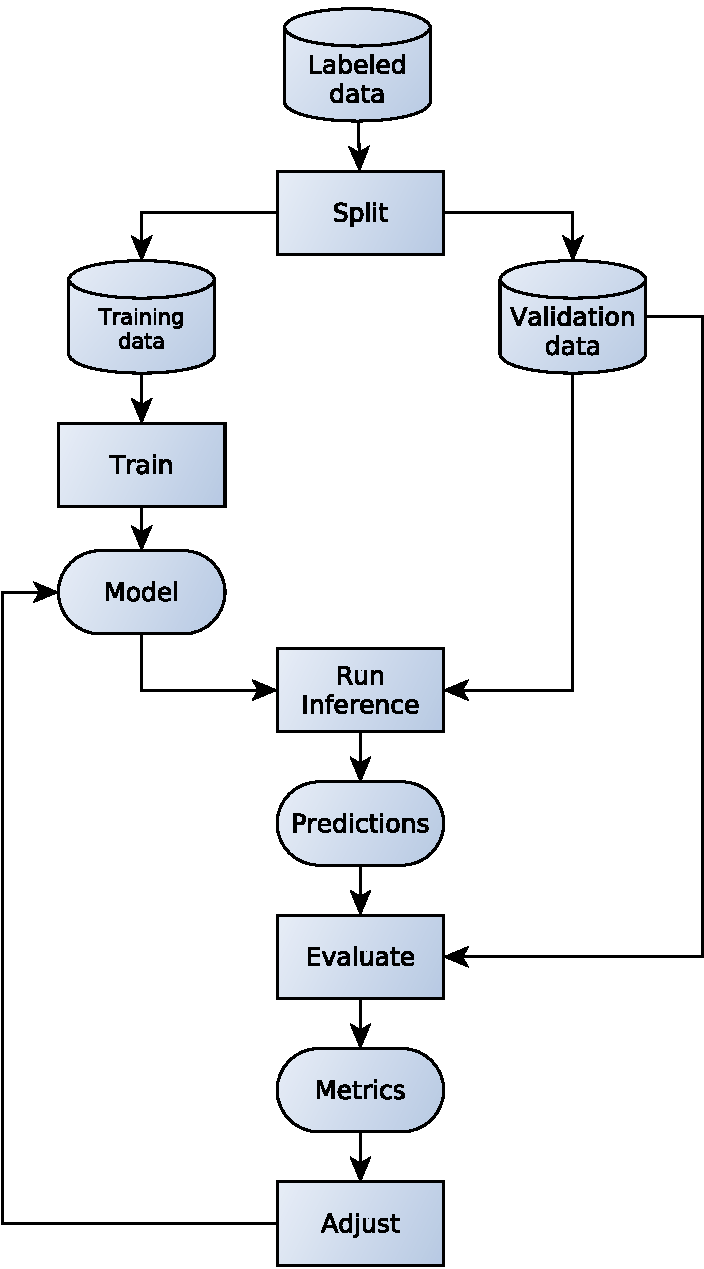
\includegraphics[width=\linewidth,height=0.75\textheight,keepaspectratio]{images/supervised_learning.pdf}
  \end{figure}
\end{frame}

\begin{frame}{Supervised learning}
  \begin{figure}
	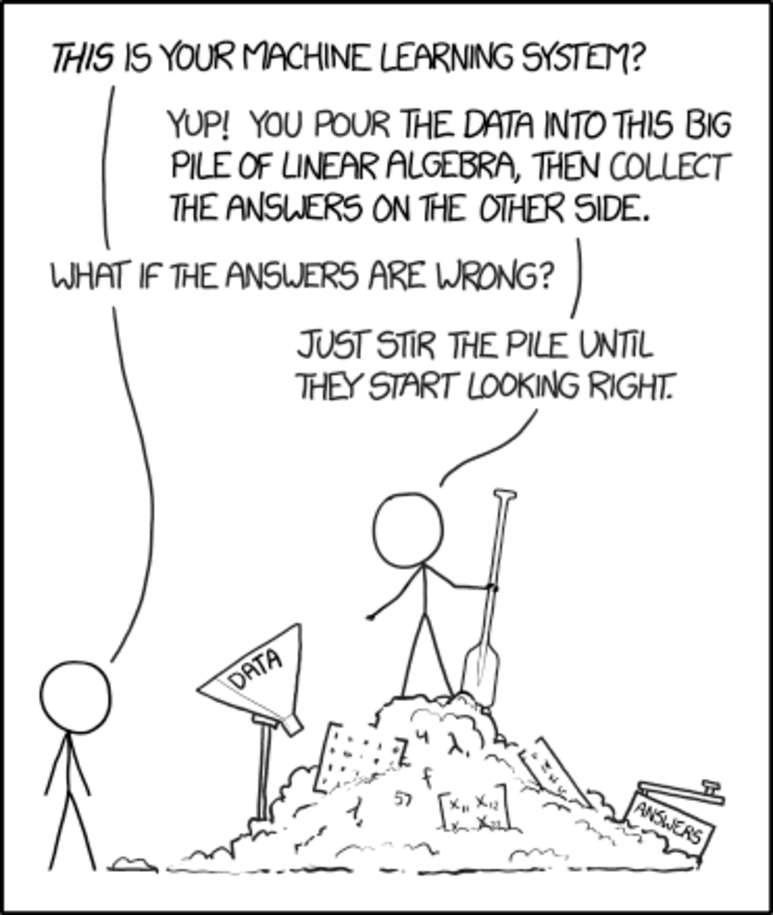
\includegraphics[width=\linewidth,height=0.8\textheight,keepaspectratio]{images/xkcd_machine_learning.pdf}
	\caption{xkcd.com}
  \end{figure}
\end{frame}

\begin{frame}{Neural network (NN)}
  \begin{figure}
	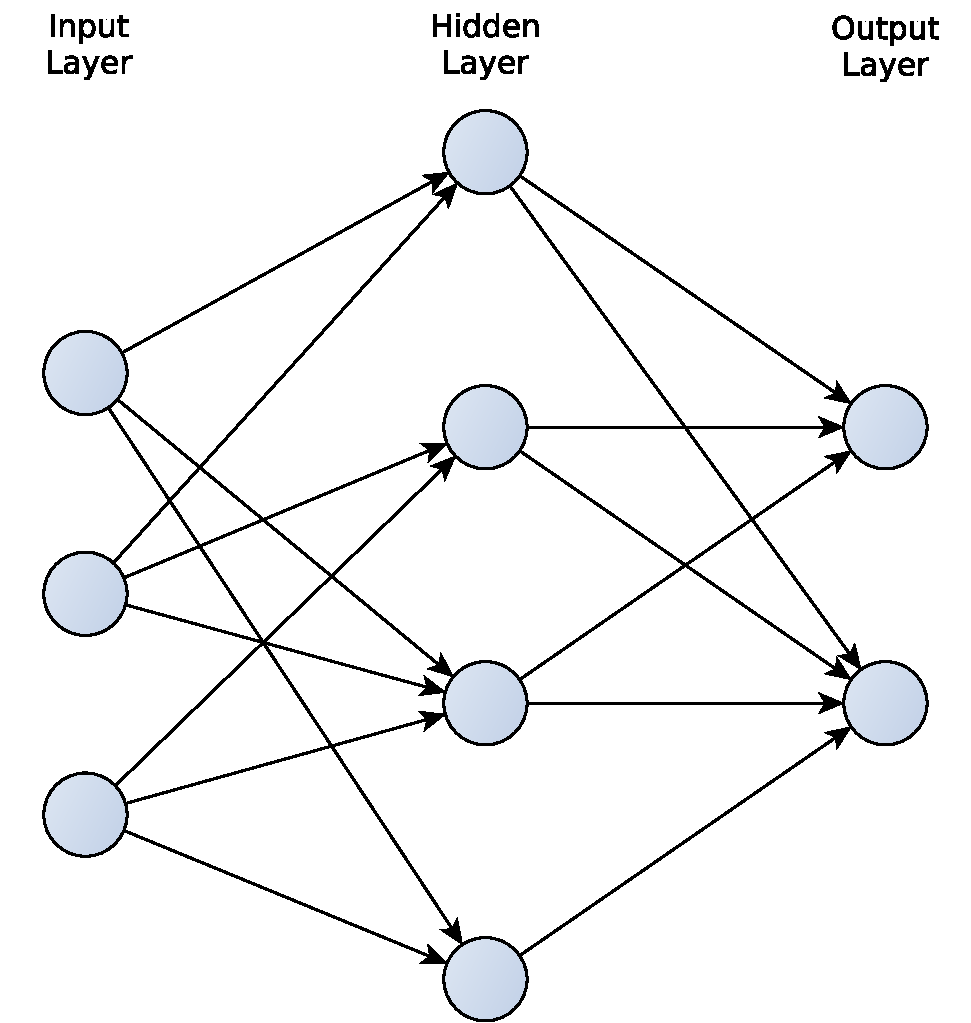
\includegraphics[width=\linewidth,height=0.75\textheight,keepaspectratio]{images/neural_network.pdf}
  \end{figure}
\end{frame}

\begin{frame}{Convolutional neural network (CNN)}
  \begin{itemize}
	\item Efficient in image classification
	\item A convolutional layer can apply filters to detect:
	  \begin{itemize}
		\item Edges
		\item Shapes
		\item Objects
	  \end{itemize}
  \end{itemize}
\end{frame}

\begin{frame}{Hardware setup}
  \begin{itemize}
	\item Raspberry Pi 4 model B:
	  \begin{itemize}
		\item Quad core Cortex-A72 (ARM v8) 64-bit SoC @ 1.8GHz
		\item 4GB RAM
	  \end{itemize}
	\item 8GB microSD card
	\item Raspberry Pi Camera module 3
  \end{itemize}
  \begin{figure}
	\includegraphics[width=\linewidth,height=\textheight,keepaspectratio]{images/rpi.pdf}
  \end{figure}
\end{frame}

\begin{frame}{Software dependencies}
  \begin{itemize}
	\item TensorFlow Lite
	\item OpenCV
  \end{itemize}
\end{frame}

\begin{frame}{MobileNet pre-trained model}
  \begin{itemize}
	\item CNN architecture created by Google
	\item Accepts 224x224-pixel images, with 3 color channels per pixel (RGB)
	\item Trained on 1000 classes
	\item Labels are stored separate from the model:
	  \begin{itemize}
		\item \texttt{labels\_mobilenet\_quant\_v1\_224.txt} (11KB)
		\item \texttt{mobilenet\_v1\_1.0\_224\_quant.tflite} (4.1MB)
	  \end{itemize}
  \end{itemize}
\end{frame}

\begin{frame}{Image classification algorithm}
  \begin{enumerate}
	\item Load model and labels
	\item Build interpreter
	\item Allocate input and output tensors
	\item Read image
	\item Resize image
	\item Copy resized image to input tensor
	\item Run inference
	\item Extract results from output tensor
  \end{enumerate}
\bigskip
Steps 1-3 represent the initialization phase \\
Steps 4-8 can be repeated multiple times
\end{frame}

\begin{frame}[fragile]{1. Load model and labels}
  \lstset{basicstyle=\ttfamily\small, numbers=left, columns=fullflexible}
  \begin{lstlisting}
// defined and properly initialized elsewhere:
// const char *model_path;
// const char *labels_path;

std::unique_ptr<tflite::FlatBufferModel> model{
  tflite::FlatBufferModel::BuildFromFile(model_path)
};

std::ifstream labels_ifs{labels_path};
std::string label;
std::vector<std::string> labels;
while (getline(labels_ifs, label)) {
  labels.push_back(std::move(label));
}
  \end{lstlisting}
\end{frame}

\begin{frame}[fragile]{2. Build interpreter}
  \lstset{basicstyle=\ttfamily\small, numbers=left, columns=fullflexible}
  \begin{lstlisting}
// defined and properly initialized elsewhere:
// std::unique_ptr<tflite::FlatBufferModel> model;
// int num_threads;

tflite::ops::builtin::BuiltinOpResolver resolver;
tflite::InterpreterBuilder builder{*model, resolver};

builder.SetNumThreads(num_threads);

std::unique_ptr<tflite::Interpreter> interpreter;
builder(&interpreter);
  \end{lstlisting}
\end{frame}

\begin{frame}[fragile]{3. Allocate input and output tensors}
  \lstset{basicstyle=\ttfamily\small, numbers=left, columns=fullflexible}
  \begin{lstlisting}
// defined and properly initialized elsewhere:
// std::unique_ptr<tflite::Interpreter> interpreter;

interpreter->AllocateTensors();
  \end{lstlisting}
\end{frame}

\begin{frame}[fragile]{4. Read image}
  \lstset{basicstyle=\ttfamily\small, numbers=left, columns=fullflexible}
  \begin{lstlisting}
// defined and properly initialized elsewhere:
// const char *image_path;

cv::Mat image{cv::imread(image_path)};
  \end{lstlisting}
\end{frame}

\begin{frame}[fragile]{5. Resize image}
  \lstset{basicstyle=\ttfamily\small, numbers=left, columns=fullflexible}
  \begin{lstlisting}
// defined and properly initialized elsewhere:
// cv::Mat image;
// int required_image_width;
// int required_image_height;

cv::Mat resized_image;
cv::resize(
  image,
  resized_image,
  cv::Size{required_image_width, required_image_height}
);
  \end{lstlisting}
\end{frame}

\begin{frame}[fragile]{6. Copy resized image to input tensor}
  \lstset{basicstyle=\ttfamily\small, numbers=left, columns=fullflexible}
  \begin{lstlisting}
// defined and properly initialized elsewhere:
// std::unique_ptr<tflite::Interpreter> interpreter;
// cv::Mat resized_image;

std::memcpy(
  interpreter->typed_input_tensor<uint8_t>(0),
  resized_image.data,
  resized_image.total() * resized_image.elemSize()
);
  \end{lstlisting}
\end{frame}

\begin{frame}[fragile]{7. Run inference}
  \lstset{basicstyle=\ttfamily\small, numbers=left, columns=fullflexible}
  \begin{lstlisting}
// defined and properly initialized elsewhere:
// std::unique_ptr<tflite::Interpreter> interpreter;

interpreter->Invoke();
  \end{lstlisting}
\end{frame}

\begin{frame}[fragile]{8. Extract results from output tensor}
  \lstset{basicstyle=\ttfamily\small, numbers=left, columns=fullflexible}
  \begin{lstlisting}
// defined and properly initialized elsewhere:
// std::unique_ptr<tflite::Interpreter> interpreter;
// std::vector<std::string> labels;

std::span<uint8_t> outputs{
  interpreter->typed_output_tensor<uint8_t>(0),
  labels.size()
};

std::vector<float> probabilities;
probabilities.reserve(labels.size());
for (auto output : outputs) {
  probabilities.push_back(
    1.0f * output / std::numeric_limits<uint8_t>::max()
  );
}
  \end{lstlisting}
\end{frame}

\begin{frame}{Demo}
  \begin{figure}
	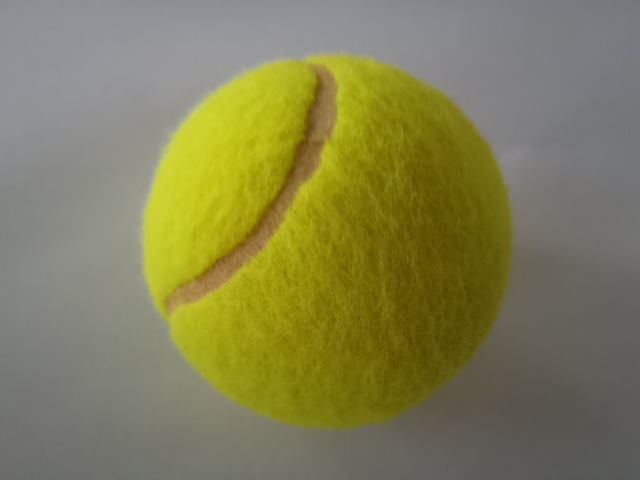
\includegraphics[width=0.5\linewidth,height=0.5\textheight,keepaspectratio]{../images/tennis_ball_input.jpeg}%
	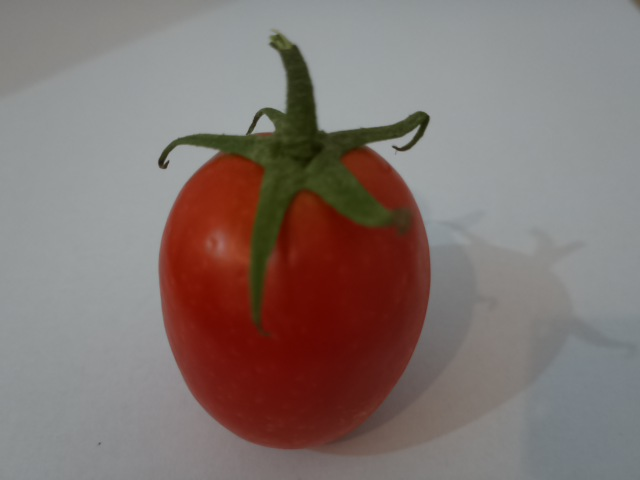
\includegraphics[width=0.5\linewidth,height=0.5\textheight,keepaspectratio]{../images/tomato.jpeg}
  \end{figure}
  \ttfamily \$ libcamera-jpeg --width=640 --height=480 -o out.jpeg
\end{frame}

\begin{frame}{Demo - Good results}
  \begin{figure}
	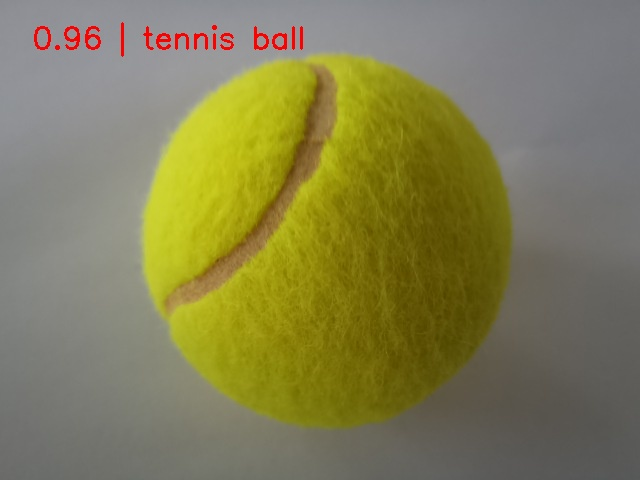
\includegraphics[width=\linewidth,height=0.5\textheight,keepaspectratio]{images/tennis_ball_output.jpeg}
  \end{figure}
  \ttfamily 0.96 | tennis ball
\end{frame}

\begin{frame}{Demo - Bad results}
  \begin{figure}
	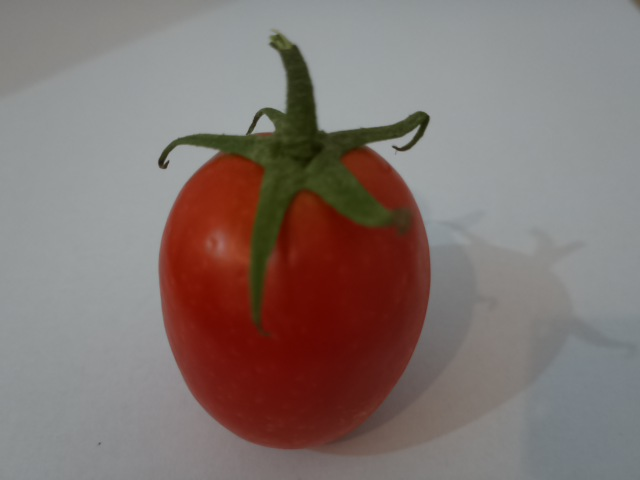
\includegraphics[width=\linewidth,height=0.5\textheight,keepaspectratio]{../images/tomato.jpeg}
  \end{figure}
  \ttfamily 0.30 | vase \\
  \ttfamily 0.25 | bell pepper \\
  \ttfamily ambiguous results
\end{frame}

\begin{frame}{Demo - Bad results explanation}
  \ttfamily \$ grep "tomato" labels\_mobilenet\_quant\_v1\_224.txt \\
  \ttfamily \$
\end{frame}

\begin{frame}{Performance}
  \begin{itemize}
	\item Compilation duration (on Raspberry Pi): 35s
	\item Binary size: 67KB
	\item Running duration: 1s
  \end{itemize}
  \begin{table}
    {\tiny
	\begin{tabular}{|c|c|}
	  \hline
		\textbf{Number of threads} & \textbf{Inference duration (ms)} \\
	  \hline
		1 & 102 \\
	  \hline
		2 & 56 \\
	  \hline
		3 & 41 \\
	  \hline
		4 & 33 \\
	  \hline
		5 & 110 \\
	  \hline
	\end{tabular}
	}
  \end{table}
  \begin{figure}
	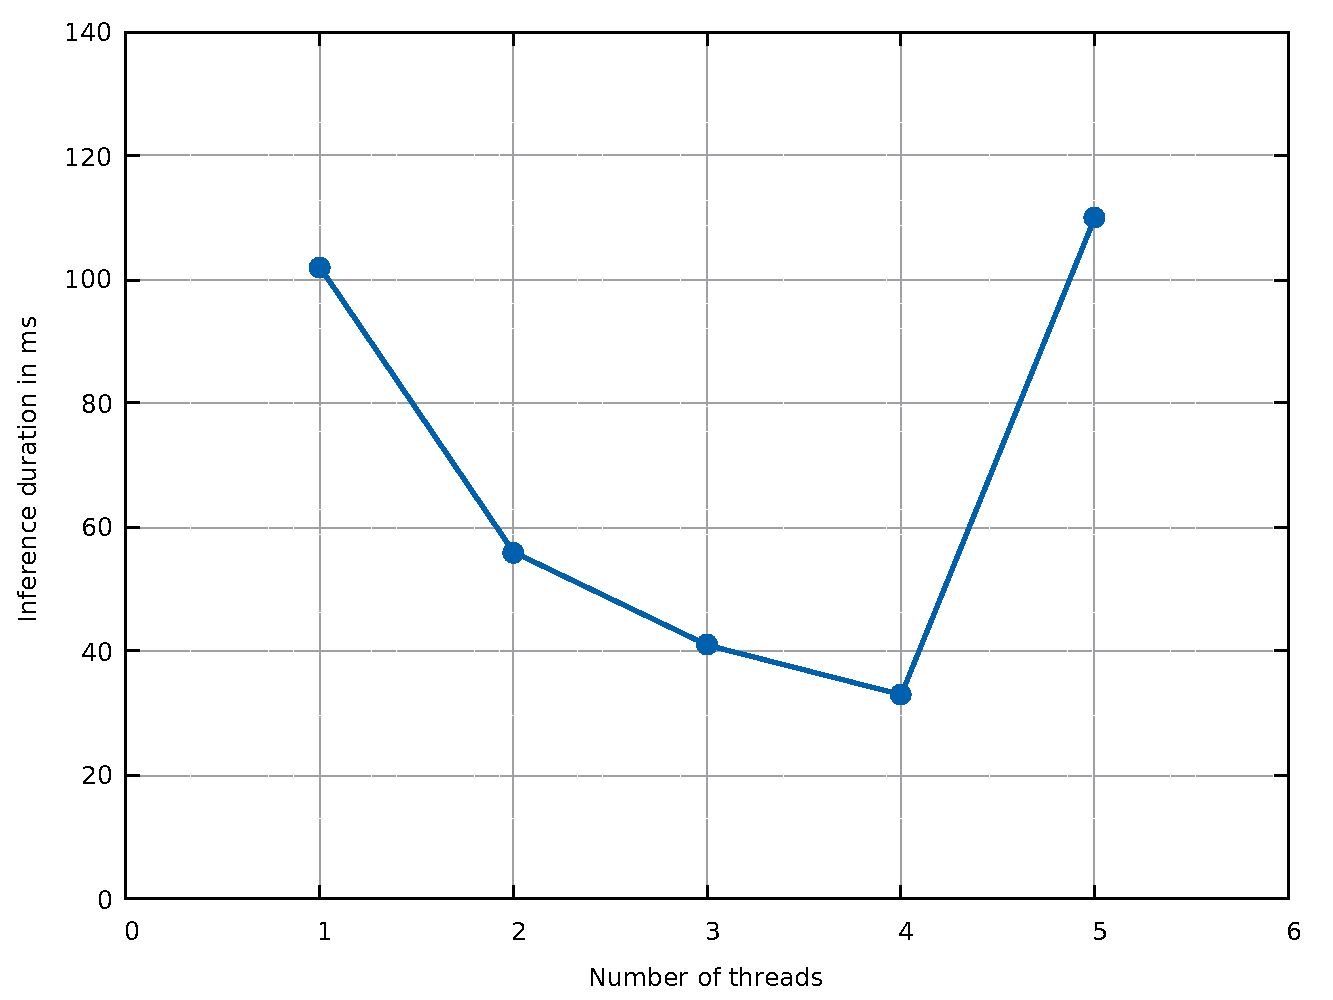
\includegraphics[width=\linewidth,height=0.45\textheight,keepaspectratio]{images/inference_duration.pdf}
  \end{figure}
  \begin{itemize}
	\item Memory consumption with 4 threads: 93MB
  \end{itemize}
\end{frame}

\begin{frame}{Comparision with Python}
Comparision made with TensorFlow Lite's \texttt{label\_image.py}
  \begin{table}
	\begin{tabular}{c|c|c|}
	  \cline{2-3}
		& \textbf{C++} & \textbf{Python} \\
	  \hline
		\multicolumn{1}{|c|}{\textbf{Running duration (s)}} & 1 & 7 \\
	  \hline
	\end{tabular}
  \end{table}
  \begin{table}
	\begin{tabular}{|c|c|c|}
	  \hline
		\textbf{Number of threads} & \multicolumn{2}{c|}{\textbf{Inference duration (ms)}} \\
	  \cline{2-3}
		& \hspace{0.35cm} \textbf{C++} \hspace{0.35cm} & \textbf{Python} \\
	  \hline
		1 & 102 & 118 \\
	  \hline
		2 & 56 & 62 \\
	  \hline
		3 & 41 & 42 \\
	  \hline
		4 & 33 & 33 \\
	  \hline
		5 & 110 & 170 \\
	  \hline
	\end{tabular}
  \end{table}
  \begin{table}
	\begin{tabular}{c|c|c|}
	  \cline{2-3}
		& \textbf{C++} & \textbf{Python} \\
	  \hline
		\multicolumn{1}{|c|}{\textbf{Memory consumption with 4 threads (MB)}} & 93 & 320 \\
	  \hline
	\end{tabular}
  \end{table}
\end{frame}

